\let\lesson\undefined
\newcommand{\lesson}{\phantomlesson{Bài 19.}}
\setcounter{section}{2}
\section{Trắc nghiệm}
\ANSMCQ
{	\begin{center}
		\begin{tabular}{|m{2.8em}|m{2.8em}|m{2.8em}|m{2.8em}|m{2.8em}|m{2.8em}|m{2.8em}|m{2.8em}|m{2.8em}|m{2.8em}|}
			\hline
			1.B  & 2.A  & 3.D  & 4.A  & 5.B  & 6.C  & 7.B  & 8.C  & 9.B  & 10.A  \\
			\hline
			11.B  & 12.B  & 13.B  & 14.A  & 15.C  & &  &   &   &  \\
			\hline
		\end{tabular}
	\end{center}
}
\begin{enumerate}[label=\bfseries Câu \arabic*:, leftmargin=1.5cm]
\item \mkstar{1}\\
Va chạm nào sau đây là va chạm mềm?
\begin{mcq}
	\item Quả bóng đang bay đập vào tường và nảy ra.
	\item Viên đạn đang bay xuyên vào và nằm gọn trong bao cát.
	\item Viên đạn xuyên qua một tấm bia trên đường bay của nó.
	\item Quả bóng tennis đập xuống sân thi đấu.
\end{mcq}
\hideall{
\textbf{Đáp án B.}
}


\item \mkstar{1}\\
{Chọn câu phát biểu \textbf{sai}?
\begin{mcq}
	\item Hệ vật – Trái Đất luôn được coi là hệ kín.
	\item Hệ vật – Trái Đất chỉ gần đúng là hệ kín.
	\item Trong các vụ nổ, hệ vật có thể coi như gần đúng là hệ kín trong thời gian ngắn xảy ra hiện tượng.
	\item Trong va chạm, hệ vật có thể coi gần đúng là hệ kín trong thời gian ngắn xảy ra va chạm.
\end{mcq}
}
\hideall{
\textbf{Đáp án A.}\\
}

\item \mkstar{2}\\
{Sở dĩ khi bắn súng trường (quan sát hình ảnh) các chiến sĩ phải tì vai vào báng súng vì hiện tượng giật lùi của súng có thể gây chấn thương cho vai. Hiện tượng súng giật lùi trên trên liên quan đến 
	\begin{center}
		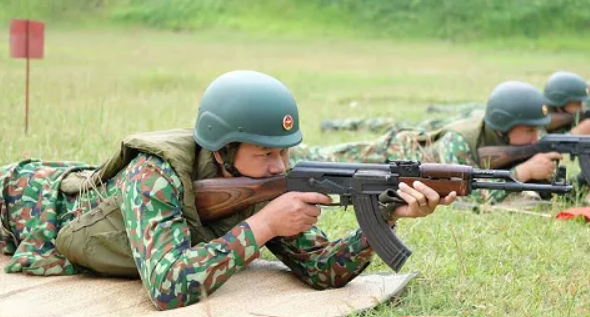
\includegraphics[width=0.3\linewidth]{../figs/VN10-2023-PH-TP030-P-1}
	\end{center}
\begin{mcq}(2)
	\item chuyển động theo quán tính.
	\item chuyển động do va chạm.
	\item chuyển động ném ngang.
	\item chuyển động bằng phản lực.
\end{mcq}
}
\hideall{
\textbf{Đáp án D.}
}

\item \mkstar{2}\\
{Quả cầu A khối lượng $m_1$ chuyển động với vận tốc $\vec v_1$ va chạm vào quả cầu B khối lượng $m_2$ đứng yên. Sau va chạm, cả hai quả cầu có cùng vận tốc $v$. Ta có
	\begin{mcq}(2)
		\item $m_1\vec v_1=\left(m_1+m_2\right)\vec v$.
		\item $m_1\vec v_1=-m_2\vec v$.
		\item $m_1\vec v_1=m_2\vec v_2$.
		\item $m_1\vec v_1=\dfrac{1}{2}\left(m_1+m_2\right)\vec v_2$.
	\end{mcq}

}
\hideall{
\textbf{Đáp án A.}
}



	\item \mkstar{2}
	
	
	{Một vật có khối lượng $m$ chuyển động với vận tốc $\SI{3}{m/s}$ đến va chạm với một vật có khối lượng  $2m$ đang đứng yên. Coi va chạm giữa hai vật là mềm. Sau va chạm, hai vật dính nhau và chuyển động với cùng vận tốc 
		
		\begin{mcq}(4)
			\item $\SI{2}{m/s}$. 
			\item $\SI{1}{m/s}$.
			\item $\SI{3}{m/s}$.
			\item $\SI{4}{m/s}$.
		\end{mcq}
	}
	
	\hideall
	{	
		\textbf{Đáp án: B.}
		
		Hệ hai vật ngay khi va chạm mềm là một hệ kín nên động lượng của hệ được bảo toàn:
		
		$$m_1\vec v_1 + m_2\vec v_2 = (m_1+m_2)\vec v.$$
		
		Do $v_2 = 0.$
		
		Suy ra:
		
		$$ v = \dfrac{m_1v_1}{m_1+m_2} = \dfrac{3m}{m+2m} = \SI{1}{m/s}.$$
		
	}

	\item \mkstar{2}
	
	
	{Chiếc xe chạy trên đường ngang với vận tốc $\SI{20}{m/s}$ va chạm mềm vào một chiếc xe khác đang đứng yên và có cùng khối lượng. Sau va chạm vận tốc hai xe là
		\begin{mcq}(2)
			\item $v_1 = 0; v_2 = \SI{10}{m/s}.$ 
			\item $v_1 = v_2 = \SI{5}{m/s}.$ 
			\item $v_1 = v_2 = \SI{10}{m/s}.$
			\item $v_1 = v_2 = \SI{20}{m/s}.$
		\end{mcq}
	}
	
	\hideall
	{	\textbf{Đáp án: C.}
		
		Áp dụng định luật bảo toàn động lượng cho hai xe ngay trước và sau va chạm ta có:
		
		$$\vec p_1 = \vec p_2 \Leftrightarrow m\vec v = 2m \vec V \Leftrightarrow \vec V = \dfrac{\vec v}{2} $$
		Sau va chạm, hai xe tiếp tục chuyển động theo hướng cũ với tốc độ
		$$V=\dfrac{v}{2}=\SI{10}{\meter/\second}.$$
	}
	\item \mkstar{2}
	
	
	{Một đầu đạn khối lượng $\SI{5}{g}$ được bắn ra khỏi nòng của một khẩu súng khối lượng $\SI{5}{kg}$ với tốc độ $\SI{500}{m/s}$. Nếu bỏ qua khối lượng của vỏ đạn thì tốc độ giật của súng là
		\begin{mcq}(4)
			\item $\SI{5}{cm/s}$. 
			\item $\SI{0,5}{m/s}.$ 
			\item $\SI{12}{m/s}.$
			\item $\SI{50}{cm/s}.$ 
		\end{mcq}
	}
	
	\hideall
	{
		\textbf{Đáp án: B.}
		
Áp dụng định luật bảo toàn động lượng cho đạn và súng ngay trước và sau khi bắn:
$$\vec 0=m_\text{s}\vec v_\text{s}+m_\text{đ}\vec v_\text{đ}\Rightarrow \vec v_\text{s}=-\dfrac{m_\text{đ}}{m_\text{s}}\cdot\vec v_\text{đ}$$
Sau khi bắn, súng giật lùi trở lại với tốc độ $v_\text{s}=\dfrac{m_\text{đ}}{m_\text{s}}\cdot v_\text{đ}=\SI{0.5}{\meter/\second}.$
		
	}
	\item \mkstar{2}
	
	
	{Khối lượng súng là $\SI{4}{kg}$ và của đạn là $\SI{50}{g}$. Lúc thoát khỏi nòng súng, đạn có tốc độ $\SI{800}{m/s}$. Tốc độ giật lùi của súng là
		\begin{mcq}(4)
			\item $\SI{6}{m/s}$. 
			\item $\SI{7}{m/s}$. 
			\item $\SI{10}{m/s}$. 
			\item $\SI{12}{m/s}$. 
		\end{mcq}
	}
	
	\hideall
	{	\textbf{Đáp án: C.}
		
	Áp dụng định luật bảo toàn động lượng cho đạn và súng ngay trước và sau khi bắn:
	$$\vec 0=m_\text{s}\vec v_\text{s}+m_\text{đ}\vec v_\text{đ}\Rightarrow \vec v_\text{s}=-\dfrac{m_\text{đ}}{m_\text{s}}\cdot\vec v_\text{đ}$$
	Sau khi bắn, súng giật lùi trở lại với tốc độ $v_\text{s}=\dfrac{m_\text{đ}}{m_\text{s}}\cdot v_\text{đ}=\SI{10}{\meter/\second}.$
	}

	\item \mkstar{2}
	
	
	{Một hòn bi khối lượng $m$ đang chuyển động với vận tốc $v$ đến va chạm mềm vào hòn bi thứ 2 khối lượng $3m$ đang nằm yên. Vận tốc hai viên bi sau va chạm là
		\begin{mcq}(4)
			\item $\dfrac{v}{3}.$
			\item $\dfrac{v}{4}.$ 
			\item $\dfrac{3v}{5}.$
			\item $\dfrac{v}{2}.$
		\end{mcq}
	}
	
	\hideall
	{	
		\textbf{Đáp án: B.}
		
		Áp dụng định luật bảo toàn động lượng cho hệ hai vật ngay trước và sau va chạm:
		
		$$m\vec v = (m+ 3m)\vec V.$$
		
		$$ \Rightarrow \vec V = \dfrac{m\vec v}{m + 3m} = \dfrac{\vec v}{4}.$$
	}
	\item \mkstar{2}
	
	
	{Một vật khối lượng $m$ đang chuyển động theo phương ngang với vận tốc $v$ thì va chạm vào vật khối lượng $4m$ đang đứng yên. Sau va chạm, hai vật dính vào nhau và chuyển động với cùng vận tốc. Bỏ qua ma sát, vận tốc của hệ sau va chạm là 
		\begin{mcq}(4)
			\item $\dfrac{v}{5}.$
			\item $v.$
			\item $5v.$
			\item $\dfrac{v}{2}.$
		\end{mcq}
	}
	
	\hideall
	{	
		\textbf{Đáp án: A.}
		
		Áp dụng định luật bảo toàn động lượng cho hệ hai vật ngay trước và sau va chạm:
		
		$$m\vec v = (m+ 4m)\vec V.$$
		
		$$ \Rightarrow \vec V = \dfrac{m\vec v}{m + 4m} = \dfrac{\vec v}{5}.$$
	}

\item \mkstar{3}\\
{Hai viên bi có khối lượng $m_1 =\SI{50}{\gram}$ và $m_2 =\SI{80}{\gram}$ đang chuyển động ngược chiều nhau và va chạm nhau. Muốn sau va chạm $m_2$ đứng yên còn $m_1$ chuyển động theo chiều ngược lại với tốc độ như cũ. Cho biết $v_1 =\SI{2}{\meter/\second}$ thì tốc độ của $m_2$ trước va chạm bằng
	\begin{mcq}(4)
		\item $\SI{1}{\meter/\second}$.
		\item $\SI{2.5}{\meter/\second}$.
		\item $\SI{3}{\meter/\second}$.
		\item $\SI{2}{\meter/\second}$.
	\end{mcq}

}
\hideall{
\textbf{Đáp án B.}\\
Áp dụng định luật bảo toàn động lượng cho hệ vật $m_1$ và $m_2$ ngay trước và sau va chạm:
$$m_1\vec v_1+m_2\vec v_2=m_1\overrightarrow{v'_1}+m_2\overrightarrow{v'_2}$$
Chiếu lên chiều chuyển động ban đầu của vật $m_1$:
$$m_1v_1-m_2v_2=-m_1v_1\Rightarrow v_2=\dfrac{2m_1v_1}{m_2}=\dfrac{2\cdot\left(\SI{0.05}{\kilogram}\right)\cdot\left(\SI{2}{\meter/\second}\right)}{\SI{0.08}{\kilogram}}=\SI{2.5}{\meter/\second}.$$
}

	\item \mkstar{3}


{
	Một viên đạn đang bay với tốc độ $\SI{10}{m/s}$ thì nổ thành hai mảnh. Mảnh thứ nhất chiếm $60\%$ khối lượng của  đạn và tiếp tục bay theo hướng ban đầu của đạn với tốc độ $\SI{25}{m/s}$. Tốc độ và hướng chuyển động của mảnh thứ hai là 
	\begin{mcq}(2)
		\item $\SI{12,5}{m/s}$; theo hướng viên đạn ban đầu. 
		\item $\SI{12,5}{m/s}$; ngược hướng viên đạn ban đầu.
		\item $\SI{6,25}{m/s}$; theo hướng viên đạn ban đầu. 
		\item $\SI{4}{m/s}$; ngược hướng viên đạn ban đầu.
	\end{mcq}
}

\hideall
{	
	\textbf{Đáp án: B.}
	
	Hệ viên đạn (hai mảnh đạn) ngay khi nổ là một hệ kín nên động lượng hệ được bảo toàn
	
	$$m\vec v = m_1 \vec v_1 + (m-m_1)\vec v_2.$$
	
	Do $\vec v_1$ cùng chiều $\vec v$.
	
	Nên 
	
	$$v_2 = \dfrac{mv - m_1v_1}{m-m_1} = -\SI{12,5}{m/s}.$$
	
	Dấu (-) chứng tỏ mảnh đạn thứ 2 sẽ chuyển động ngược chiều chuyển động ban đầu của viên đạn và mảnh đạn thứ nhất.
}


\item \mkstar{3}\\
{Một viên đạn khối lượng $\SI{1}{\kilogram}$ đang bay thẳng đứng lên cao với tốc độ $\SI{400}{\meter/\second}$ thì nổ thành hai mảnh có khối lượng bằng nhau. Biết mảnh I bay với tốc độ $\SI{400}{\meter/\second}$ theo phương lệch một góc $\SI{60}{\degree}$ so với đường thẳng đứng. Mảnh II bay theo phương hợp với phương bay của mảnh I một góc
	\begin{mcq}(4)
		\item $\SI{75}{\degree}$.
		\item $\SI{90}{\degree}$.
		\item $\SI{30}{\degree}$.
		\item $\SI{120}{\degree}$.
	\end{mcq}
}
\hideall{
\textbf{Đáp án B.}\\
Động lượng ban đầu của viên đạn:
$$p=mv=\SI{400}{\kilogram\cdot\meter/\second}$$
Động lượng của mảnh I:
$$p_1=m_1v_1=\SI{200}{\kilogram\cdot\meter/\second}$$
Áp dụng định luật bảo toàn động lượng của các mảnh vỡ ngay trước và sau khi đạn nổ:
$$\vec p=\vec p_1+\vec p_2$$
$$\Rightarrow \vec p_2=\vec p-\vec p_1$$
$$\Leftrightarrow p_2=\sqrt{p^2+p^2_1-2pp_1\cos\SI{60}{\degree}}=\xsi{200\sqrt{3}}{\kilogram\cdot\meter/\second}$$
Vì $p^2_1+p^2_2=p^2\Rightarrow \vec p_1\bot \vec p_2$.
}

	\item \mkstar{3}
	
	
	{Một người có khối lượng $m_1=\SI{60}{kg}$ nhảy từ một chiếc xe có khối lượng $m_2 = \SI{80}{kg}$ đang chuyển động theo phương ngang với tốc độ $v = \SI{3}{m/s}$. Biết tốc độ nhảy của người đối với xe lúc xe chưa thay đổi vận tốc là $\SI{4}{m/s}$. Tốc độ của xe sau khi người ấy nhảy ngược chiều với chiều chuyển động của xe là
		\begin{mcq}(4)
			\item $\SI{6}{m/s}.$
			\item $\SI{5}{m/s}.$ 
			\item $\SI{4}{m/s}.$
			\item $\SI{3}{m/s}.$
		\end{mcq}
	}
	
	\hideall
	{	
		\textbf{Đáp án: A.}\\
		Gọi:
		\begin{itemize}
			\item (1) người;
			\item (2) xe;
			\item (0) đất.
		\end{itemize}
	Ta có: $v_{20}=\SI{3}{\meter/\second}$, $v'_{12}=\SI{4}{\meter/\second}$.\\
	Áp dụng định luật bảo toàn động lượng cho hệ người và xe ngay trước và sau khi người nhảy:
	\begin{eqnarray*}
		\left(m_1+m_2\right)\overrightarrow{v_{20}}&=&m_1\overrightarrow{v'_{10}} +m_2\overrightarrow{v'_{20}}\\
		\Leftrightarrow \left(m_1+m_2\right)\overrightarrow{v_{20}}&=&m_1\left(\overrightarrow{v'_{12}}+\overrightarrow{v_{20}}\right) +m_2\overrightarrow{v'_{20}}\\
		\Rightarrow m_2\overrightarrow{v_{20}}&=&m_1\overrightarrow{v'_{12}}+m_2\overrightarrow{v'_{20}} \quad (*)
	\end{eqnarray*}		
Chiếu phương trình (*) lên chiều chuyển động ban đầu của xe:
$$m_2v_{20}=-m_1v'_{12}+m_2v'_{20}\Rightarrow v'_{20}=\dfrac{m_2v_{20}+m_1v'_{12}}{m_2}$$
$$\Leftrightarrow v'_{20}=\dfrac{\left(\SI{80}{\kilogram}\right)\cdot\left(\SI{3}{\meter/\second}\right)+\left(\SI{60}{\kilogram}\right)\cdot\left(\SI{4}{\meter/\second}\right)}{\SI{80}{\kilogram}}=\SI{6}{\meter/\second}$$
	}
	
	
	\item \mkstar{4}\\
	{Ở ngã tư của hai đường vuông góc giao nhau, do đường trơn, một ô tô khối lượng $m_1=\SI{1000}{\kilogram}$ va chạm với một ô tô thứ hai khối lượng $m_2=\SI{2000}{\kilogram}$ đang chuyển động với tốc độ $v_2=\SI{3}{\meter/\second}$. Sau va chạm, hai ô tô mắc vào nhau và chuyển động theo hướng làm một góc $\SI{45}{\degree}$ so với hướng chuyển động ban đầu của mỗi ô tô. Tìm tốc độ $v_1$ của ô tô thứ nhất trước va chạm và tốc độ $v$ của hai ô tô sau va chạm.
	\begin{mcq}(2)
		\item $v_1=\SI{3}{\meter/\second}$, $v=\xsi{3\sqrt{2}}{\meter/\second}$.
		\item $v_1=\SI{3}{\meter/\second}$, $v=\SI{2.83}{\meter/\second}$.
		\item $v_1=\SI{6}{\meter/\second}$, $v=\SI{2.83}{\meter/\second}$.
		\item $v_1=\SI{6}{\meter/\second}$, $v=\SI{4.5}{\meter/\second}$.
	\end{mcq}
}
\hideall{
	\textbf{Đáp án C.}\\
	Áp dụng định luật bảo toàn động lượng cho hai ô tô ngay trước và sau khi va chạm:
	$$\vec p_1+\vec p_2=\overrightarrow{p'}$$
	\begin{center}
		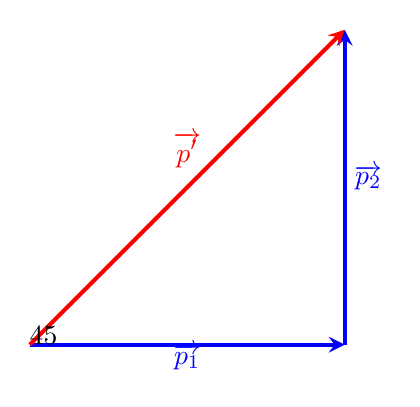
\begin{tikzpicture}
			\coordinate (O) at (0,0);
			\coordinate (A) at (4,0);
			\coordinate (B) at (4,4);
			\draw[-stealth,line width=1.5, blue] (O) -- (A);
			\draw[-stealth,line width=1.5, blue] (A) -- (B);
			\draw[-stealth,line width=1.5, red] (O) -- (B);
			\node[label={[blue,below]90:$\overrightarrow{p_1}$}] at (2,0){};	
			\node[label={[blue,right]90:$\overrightarrow{p_2}$}] at (4,2){};	
			\node[label={[red,above]90:$\overrightarrow{p'}$}] at (2,2){};	
			\tkzMarkAngle[size=0.75cm,color=cyan](A,O,B);
			\tkzLabelAngle[color=black,pos=1.2](A,O,B){$\SI{45}{\degree}$}
		\end{tikzpicture}
	\end{center}
	Động lượng ban đầu của ô tô thứ nhất:
	$$p_1=\dfrac{p_2}{\tan\SI{45}{\degree}}=p_2$$
	$$\Leftrightarrow m_1v_1=m_2v_2\Rightarrow v_1=\dfrac{m_2v_2}{m_1}=\dfrac{\left(\SI{2000}{\kilogram}\right)\cdot\left(\SI{3}{\meter/\second}\right)}{\SI{1000}{\kilogram}}=\SI{6}{\meter/\second}$$
	Tốc độ của hai xe sau va chạm:
	$$p=\sqrt{p^2_1+p^2_2}=p_2\sqrt{2}$$
	$$\Leftrightarrow \left(m_1+m_2\right)v=m_2v_2\sqrt{2}$$
	$$\Rightarrow v=\dfrac{m_2v_2\sqrt{2}}{m_1+m_2}=\dfrac{\left(\SI{2000}{\kilogram}\right)\cdot\left(\SI{3}{\meter/\second}\right)\sqrt{2}}{\SI{3000}{\kilogram}}\approx\SI{2.83}{\meter/\second}.$$
}
\end{enumerate}
\section{Tự luận}
\begin{enumerate}[label=\bfseries Câu \arabic*:, leftmargin=1.5cm]
	
	
	\item \mkstar{2}
	
	
	{
		Vật $\SI{200}{\gram}$ chuyển động với tốc độ $\SI{6}{\meter/\second}$ đến va chạm với vật $\SI{50}{\gram}$ chuyển động với tốc độ $\SI{4}{\meter/\second}$. Sau va chạm vật $\SI{200}{\gram}$ giữ nguyên hướng và chuyển động với tốc độ bằng nửa vận tốc ban đầu. Tính tốc độ của vật còn lại trong các trường hợp sau:
		\begin{enumerate}[label=\alph*)]
			\item Trước va chạm hai vật chuyển động cùng chiều.
			\item Trước va chạm hai vật chuyển động ngược chiều.
		\end{enumerate}
	}
	
	\hideall
	{	
		\begin{enumerate}[label=\alph*)]
			\item Trước va chạm hai vật chuyển động cùng chiều.
			
			Áp dụng định luật bảo toàn động lượng cho hai vật ngay trước và sau va chạm:
			\begin{equation}
				\label{eq:30-P.1}
				m_1\vec v_1+m_2\vec v_2=m_1\overrightarrow{v'_1}+m_2\overrightarrow{v'_2}
			\end{equation}
		Chiếu phương trình (\ref{eq:30-P.1}) lên chiều chuyển động ban đầu của vật 1:
			$$m_1v_1 + m_2 v_2 = m_1v_1' + m_2 v_2' $$
			$$\Rightarrow v_2'=\dfrac{m_1v_1+m_2v_2-\dfrac{m_1v_1}{2}}{m_2}=\dfrac{\dfrac{\left(\SI{0.2}{\kilogram}\right)\cdot\left(\SI{6}{\meter/\second}\right)}{2}+\left(\SI{0.05}{\kilogram}\right)\cdot\left(\SI{4}{\meter/\second}\right)}{\SI{0.05}{\kilogram}}=\SI{16}{m/s}.$$
			
			\item Trước va chạm hai vật chuyển động ngược chiều.
			Áp dụng định luật bảo toàn động lượng cho hai vật ngay trước và sau va chạm:
			\begin{equation}
				\label{eq:30-P.2}
				m_1\vec v_1+m_2\vec v_2=m_1\overrightarrow{v'_1}+m_2\overrightarrow{v'_2}
			\end{equation}
			Chiếu phương trình (\ref{eq:30-P.2}) lên chiều chuyển động ban đầu của vật 1:
			$$m_1v_1 - m_2 v_2 = m_1v_1' + m_2 v_2' $$
			$$\Rightarrow v_2'=\dfrac{m_1v_1-m_2v_2-\dfrac{m_1v_1}{2}}{m_2}=\dfrac{\dfrac{\left(\SI{0.2}{\kilogram}\right)\cdot\left(\SI{6}{\meter/\second}\right)}{2}-\left(\SI{0.05}{\kilogram}\right)\cdot\left(\SI{4}{\meter/\second}\right)}{\SI{0.05}{\kilogram}}=\SI{8}{m/s}.$$
		\end{enumerate}
	}
	\item \mkstar{2}
	
	
	{
		Một vật khối lượng $\SI{0.8}{kg}$ chuyển động trên mặt phẳng ngang với tốc độ $\SI{12}{m/s}$, đến va chạm với một vật khác có khối lượng $\SI{0.2}{kg}$ đang đứng yên trên mặt phẳng ngang ấy. Sau va chạm hai vật nhập lại làm một và chuyển động với cùng tốc độ. Tính tốc độ của hai vật sau va chạm.
	}
	
	\hideall
	{	
		Áp dụng định luật bảo toàn động lượng cho hai vật ngay trước và sau va chạm:
		\begin{equation}
			\label{eq:30-P.3}
			m_1\vec v_1+m_2\vec v_2=\left(m_1+m_2\right)\vec v
		\end{equation}
	Chiếu phương trình (\ref{eq:30-P.3}) lên chiều chuyển động ban đầu của vật 1:
		$$m_1v_1= (m_1 + m_2) v \Rightarrow v=\dfrac{m_1v_1}{m_1+m_2}=\dfrac{\left(\SI{0.8}{\kilogram}\right)\cdot\left(\SI{12}{\meter/\second}\right)}{\SI{0.8}{\kilogram}+\SI{0.2}{\kilogram}}=\SI{9.6}{m/s}.$$
	}
	
	\item \mkstar{2}
	
	
	{
		Một vật khối lượng $m_1=\SI{400}{g}$ chuyển động trên mặt phẳng ngang với vận tốc $\SI{18}{km/h}$, đến va chạm với một vật khác có khối lượng $\SI{100}{g}$ đang đứng yên trên mặt phẳng ngang ấy. Sau va chạm hai vật nhập lại làm một và chuyển động với cùng vận tốc. Tính vận tốc của hai vật sau va chạm.
	}
	
	\hideall
	{	
		Áp dụng định luật bảo toàn động lượng trong va chạm mềm (hai vật dính vào nhau sau va chạm):
		$$m_1v_1 + m_2 v_2 = (m_1 + m_2) v \Rightarrow v=\SI{4}{m/s}.$$
	}
	\item \mkstar{2}
	
	
	{
		Một khẩu súng $M = \SI{4}{kg}$ bắn ra viên đạn $m = \SI{20}{g}$. Vận tốc của đạn ra khỏi nòng súng là $\SI{600}{m/s}$. Súng giật lùi với vận tốc $V$ có độ lớn là bao nhiêu?
	}
	
	\hideall
	{	
		Chọn chiều dương là chiều chuyển động của viên đạn.
		
		Áp dụng bảo toàn động lượng cho hệ đạn và súng ngay trước và sau khi bắn:
		\begin{equation}
			\label{eq:30-P.4}
			\vec 0=m\vec v+M\vec V
		\end{equation}
	$$\Rightarrow V=-\dfrac{m}{M}\cdot\vec v$$
	Súng bị giật trở lại với tốc độ:
	$$V=\dfrac{mv}{M}=\dfrac{\left(\SI{0.02}{\kilogram}\right)\cdot\left(\SI{600}{\meter/\second}\right)}{\SI{4}{\kilogram}}=\SI{3}{\meter/\second}.$$
	}
	\item \mkstar{2}
	
	
	{Một tên lửa khối lượng tổng cộng 70 tấn đang bay với tốc độ $\SI{200}{m/s}$ đối với Trái Đất thì tức thời phụt ra lượng khí 5 tấn, với tốc độ $\SI{450}{m/s}$ đối với tên lửa. Xác định vận tốc của tên lửa sau khi phụt khí ra.
	}
	
	\hideall
	{	Gọi:
		\begin{itemize}
			\item (1) khí phụt ra sau tên lửa;
			\item (2) tên lửa;
			\item (0) mặt đất.
		\end{itemize}
		Ta có: $v_{20}=\SI{200}{\meter/\second}$; $v'_{12}=\SI{450}{\meter/\second}$.
		
		Áp dụng định luật bảo toàn động lượng cho hệ tên lửa và khí ngay trước và sau khi khí phụt ra:
		\begin{eqnarray*}
			\left(m_1+m_2\right)\overrightarrow{v_{20}}&=&m_1\overrightarrow{v'_{10}}+m_2\overrightarrow{v'_{20}}\\
			\Leftrightarrow \left(m_1+m_2\right)\overrightarrow{v_{20}}&=&m_1\left(\overrightarrow{v'_{12}}+\overrightarrow{v_{20}}\right)+m_2\overrightarrow{v'_{20}}\\
			\Rightarrow m_2\overrightarrow{v_{20}}&=&m_1\overrightarrow{v'_{12}}+m_2\overrightarrow{v'_{20}} \quad (*)
		\end{eqnarray*}
		Chiếu phương trình (*) lên chiều chuyển động ban đầu của tên lửa, thu được:
		$$m_2v_{20}=-m_1v'_{12}+m_2v'_{20}$$
		$$\Rightarrow v'_{20}=\dfrac{m_2v_{20}+m_1v'_{12}}{m_2}=\dfrac{\left(\SI{65E3}{\kilogram}\right)\cdot\left(\SI{200}{\meter/\second}\right)+\left(\SI{5E3}{\kilogram}\right)\cdot\left(\SI{450}{\meter/\second}\right)}{\SI{65E3}{\kilogram}}\approx\SI{234.6}{\meter/\second}.$$
	}

\item \mkstar{3}\\
{Một ô tô con khối lượng 1,2 tấn đang chuyển động với tốc độ $\SI{25}{\meter/\second}$ thì va chạm vào đuôi của một xe tải khối lượng 9 tấn đang chạy cùng chiều với tốc độ $\SI{20}{\meter/\second}$ . Sau va chạm, ô tô con vẫn chuyển động theo hướng cũ với tốc độ $\SI{18}{\meter/\second}$.
\begin{enumerate}[label=\alph*)]
	\item Xác định vận tốc của xe tải ngay sau va chạm.
	\item Xác định phần năng lượng tiêu hao trong quá trình va chạm. Giải thích tại sao có sự tiêu hao năng lượng này.
\end{enumerate}
}
\hideall{
\begin{enumerate}[label=\alph*)]
	\item Gọi:
	\begin{itemize}
		\item $m_1$, $m_2$ lần lượt là khối lượng xe ô tô và xe tải;
		\item $v_1$, $v'_1$, $v_2$, $v'_2$ lần lượt là vận tốc của xe ô tô, xe tải trước và sau va chạm.
	\end{itemize}
Áp dụng định luật bảo toàn động lượng cho hệ ô tô và xe tải ngay trước và sau va chạm:
\begin{equation}
	\label{eq:30-P.5}
	m_1\vec v_1+m_2\vec v_2=m_1\overrightarrow{v'_1}+m_2\overrightarrow{v'_2}
\end{equation}
Chiếu (\ref{eq:30-P.5}) lên hướng chuyển động ban đầu của ô tô:
$$m_1v_1+m_2v_2=m_1v'_1+m_2v'_2\Rightarrow v'_2=\dfrac{m_1v_1+m_2v_2-m_1v'_1}{m_2}\approx\SI{20.93}{\meter/\second}.$$
Như vậy, xe ô tô tải vẫn chuyển động theo hướng cũ với tốc độ $\SI{20.93}{\meter/\second}.$
\item Năng lượng tiêu hao trong quá trình va chạm:
$$\Delta W=\dfrac{1}{2}m_1v^2_1+\dfrac{1}{2}m_2v^2_2-\left(\dfrac{1}{2}m_1v'^2_1+\dfrac{1}{2}m_2v'^2_2\right)\approx\SI{9308}{\joule}.$$
Năng lượng tiêu hao làm biến dạng kết cấu của hai xe, động năng của các mảng vỡ, nhiệt lượng ở bề mặt tiếp xúc.
	 
\end{enumerate}
}

\item \mkstar{3}\\
{Con lắc đạn đạo là thiết bị được sử dụng để đo tốc độ của viên đạn. Viên đạn được bắn vào một khúc gỗ lớn treo lơ lửng bằng dây nhẹ, không dãn. Sau khi va chạm, viên đạn ghim vào trong khối gỗ. Sau đó, toàn bộ hệ khối gỗ và viên đạn chuyển động như một con lắc lên độ cao $h$ (xem hình). Xét viên đạn có khối lượng $m_1=\SI{5}{\gram}$, khối gỗ có khối lượng $m_2=\SI{1}{\kilogram}$ và  $h=\SI{5}{\centi\meter}$. Lấy $g=\SI{9.8}{\meter/\second^2}$. Bỏ qua sức cản của không khí
	\begin{center}
		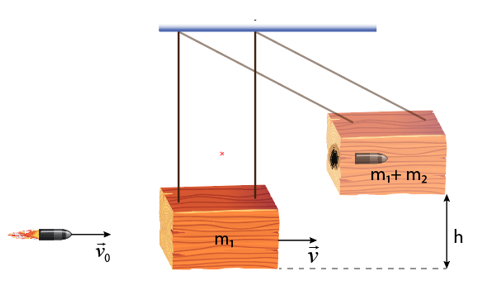
\includegraphics[width=0.35\linewidth]{../figs/VN10-2023-PH-TP030-P-2}
	\end{center}
\begin{enumerate}[label=\alph*)]
	\item Tính vận tốc của hệ sau khi viên đạn ghim vào khối gỗ.
	\item Tính tốc độ ban đầu của viên đạn.
\end{enumerate}
}
\hideall{
\begin{enumerate}[label=\alph*)]
	\item Chọn gốc thế năng tại vị trí thấp nhất của con lắc.\\
	Áp dụng định luật bảo toàn cơ năng cho hệ ngay sau khi va chạm cho đến khi con lắc đạt độ cao cực đại:
	$$\dfrac{1}{2}\left(m_1+m_2\right)v^2=\left(m_1+m_2\right)gh\Rightarrow v=\sqrt{2gh}\approx\SI{0.99}{\meter/\second}.$$
	\item Áp dụng định luật bảo toàn động lượng cho hệ khối gỗ - viên đạn ngay trước và sau va chạm:
	$$m_1\vec v_0=\left(m_1+m_2\right)\vec v\Rightarrow \vec v_0=\dfrac{\left(m_1+m_2\right)}{m_1}\cdot\vec v$$
	Tốc độ ban đầu của viên đạn:
	$$v_0=\dfrac{\left(m_1+m_2\right)v}{m_1}\approx\SI{198.99}{\meter/\second}.$$
\end{enumerate}
}

\item \mkstar{4}\\
{Một khẩu pháo được gắn chặt vào xe và xe có thể di chuyển dọc theo đường ray nằm ngang như hình. Khẩu pháo bắn ra một viên đạn khối lượng $\SI{200}{\kilogram}$ với tốc độ $\SI{125}{\meter/\second}$ theo hướng hợp với phương ngang một góc $\SI{45}{\degree}$. Biết khối lượng của khẩu pháo và xe là $\SI{5000}{\kilogram}$. Tính tốc độ giật lùi của khẩu pháo.
	\begin{center}
		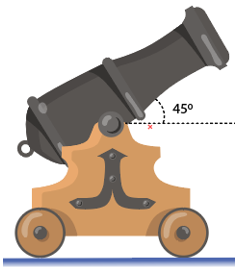
\includegraphics[width=0.25\linewidth]{../figs/VN10-2023-PH-TP030-P-3}
	\end{center}

}
\hideall{
Gọi 
\begin{itemize}
	\item $\vec v_1$, $\vec v_2$ lần lượt là vận tốc của viên đạn và khẩu pháo ngay sau khi bắn;
	\item $m_1$, $m_2$ lần lượt là khối lượng của viên đạn và khẩu pháo.
\end{itemize}
Áp dụng định luật bảo toàn động lượng cho hệ viên đạn - khẩu pháo ngay trước và sau khi bắn:
$$\vec 0=m_1\vec v_1+m_2\vec v_2\Rightarrow \vec v_2=-\dfrac{m_1\vec v_1}{m_2}$$
Nghĩa là pháo bị giật lùi cùng phương, ngược chiều vector vận tốc của đạn.\\
Tốc độ giật lùi:
$$v_2=\dfrac{m_1v_1}{m_2}=\SI{5}{\meter/\second}.$$
Tốc độ giật lùi của khẩu pháo theo phương ngang:
$$v_{2x}=v_2\cos\SI{45}{\degree}\approx\SI{3.54}{\meter/\second}.$$
}
\end{enumerate}